\documentclass[a4paper,12pt]{article}
\usepackage[brazil]{babel}
\usepackage[utf8]{inputenc}
\usepackage{indentfirst}
\usepackage{amsmath}
\usepackage{graphicx}
\usepackage{float}
\usepackage{array}
\usepackage[font=footnotesize,labelfont=bf]{caption}
\usepackage{geometry}
\usepackage{listings}
\usepackage{subcaption}
\usepackage{xcolor}
\usepackage[skins,xparse,breakable]{tcolorbox}
\usepackage{longtable}
\usepackage{minted}
\usepackage{titlesec}
\usepackage{fancyhdr}
\usepackage{setspace}
\usepackage[colorlinks=true, allcolors=black]{hyperref}

% Configurações de margens e espaçamento
\geometry{a4paper, left=3cm, right=2cm, top=3cm, bottom=2cm}
\setlength{\parindent}{1.25cm}
\onehalfspacing

% Configurações de títulos
\titleformat{\section}{\normalfont\large\bfseries}{\thesection}{1em}{}
\titleformat{\subsection}{\normalfont\bfseries}{\thesubsection}{1em}{}
\titleformat{\subsubsection}{\normalfont\itshape}{\thesubsubsection}{1em}{}

% Configurações de listagens
\renewcommand{\listingscaption}{Código}
\newenvironment{code}{\captionsetup{type=listing}}{}

% Configurações de cores
\definecolor{LightSeaGreen}{rgb}{0.1255, 0.6980, 0.6667}
\definecolor{cinza}{rgb}{0.498, 0.498, 0.498}
\definecolor{whitesmoke}{rgb}{0.96, 0.96, 0.96}

% Configurações do minted para VHDL
\setminted[VHDL]{
    style=vs,
    breaklines=true,
    mathescape=true,
    linenos=true,
    bgcolor=whitesmoke,
}

% Configurações de cabeçalho e rodapé
\pagestyle{fancy}
\fancyhf{}
\fancyhead[L]{\footnotesize{Laboratório de Sistemas Digitais - 2024/2 - Turma 2}}
\fancyhead[R]{\footnotesize{\thepage}}
\fancyfoot[C]{\footnotesize{Relatório do Experimento 2}}

\begin{document}

% Capa
\begin{titlepage}
    \begin{center}
        \vspace*{2cm}
        {\Large \textbf{Universidade de Brasília}} \\
        {\Large \textbf{Departamento de Engenharia Elétrica}} \\
        \vspace{3cm}
        {\Huge \textbf{Relatório do Experimento 2}} \\
        \vspace{2cm}
        {\Large \textbf{Laboratório de Sistemas Digitais}} \\
        \vspace{2cm}
        {\Large \textbf{Autor: Henrique Morcelles Salum}} \\
        {\Large \textbf{Matrícula: 232003008}} \\
        \vspace{2cm}
        {\Large \textbf{Brasília, 21 de outubro de 2024}}
    \end{center}
\end{titlepage}

% Sumário
\newpage
\tableofcontents
\newpage

% Introdução
\section{Introdução}
Este experimento é composto por duas tarefas, em ambas, deve-se implementar funções booleanas com VHDL e simular os circuitos lógicos implementados por meio do software ModelSim, da Intel. As especificidades de cada tarefa serão exploradas a seguir.

Na primeira, implementa-se um somador completo. Um somador completo é um circuito lógico combinacional que realiza a soma de três bits: dois bits de entrada, $A$ e $B$, e um bit adicional, $C$ (tipicamente chamado de $C_{in}$, carry-in), que representa o "vai-um" (carry-out) de uma operação anterior. Ele gera duas saídas: $S$, o resultado da soma dos três bits, e $T$ (tipicamente chamado de $C_{out}$, carry-out), o "vai-um" que pode ser gerado por essa soma. Para isso, definimos na entidade somadorCompleto os sinais de entrada $A$, $B$ e $C_{in}$ e os sinais de saída $S$ e $C_{out}$, que concatenados representam a soma dos três bits de entrada - de acordo com as definições a seguir:

\[
S = A \oplus B \oplus C_{in}
\]
\[
C_{out} = A \cdot B + A \cdot C_{in} + B \cdot C_{in}.
\]

\noindent O valor dos sinais de saída são definidos na "architecture".

Na segunda (Questão 2), deve-se implementar um multiplexador de 4 para 1, utilizando dois vetores de entrada: $S$, de dois sinais e $D$, de quatro sinais. A saída é um sinal $Y$ definido como segue:

\[
Y = D_3 \cdot \overline{S_1} \cdot \overline{S_0} + D_2 \cdot \overline{S_1} \cdot S_0 + D_1 \cdot S_1 \cdot \overline{S_0} + D_0 \cdot S_1 \cdot S_0
\]

% Teoria
\section{Teoria}
O somador completo é uma função booleana usada para realizar a adição de dois números binários. Essa função tem três entradas binárias: os dois bits de uma posição específica na representação binária dos números somados e um terceiro bit, que representa o carry-in (por isso $C_{in}$), que pode vir da adição em uma posição de ordem inferior (1 + 1 = 10, e “vai-um” para a soma na próxima posição), além de duas saídas: S, que representa o resultado da soma dos três bits de entrada e $C_{out}$, que representa o carry-out, o bit gerado para a adição na próxima posição do número binário (adição em que será o $C_{in}$).

\begin{figure}[H]
    \centering
    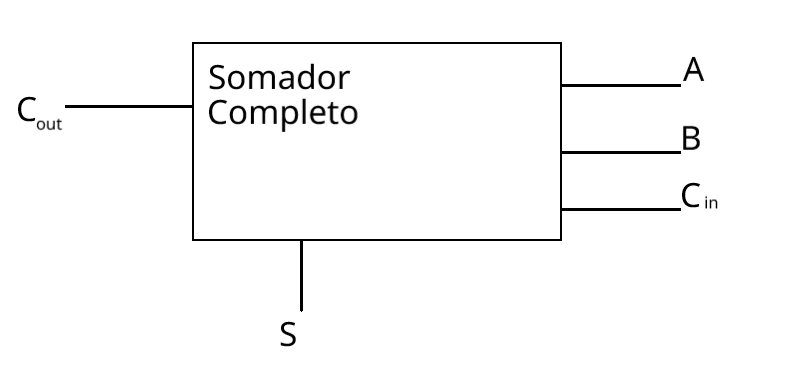
\includegraphics[width=0.75\textwidth]{./Imagens/SomadorCompleto.png}
    \caption{Representação do somador completo}
\end{figure}

Um multiplexador é um dispositivo digital que seleciona uma entre várias entradas de dados e a encaminha para uma única linha de saída. Essencialmente, o multiplexador atua como um "comutador" controlado por uma entrada de seleção, determinando qual sinal será encaminhado para a saída.

Para entender esse dispositivo, podemos separar as entradas entre entradas de dados, que são as entradas de informações a serem selecionadas, e as entradas de seleção, que são utilizadas para escolher qual das entradas de dados será enviada para a saída. O número de entradas de seleção pode ser calculado em função do número de entradas de dados pela função: 

\[
f(n) = \lceil \log_2n \rceil
\]

Nesse experimento, implementa-se, especificamente, um multiplexador 4 x 1, ou seja, com quatro entradas de dados e, consequentemente, $\log_2 4 = 2$ entradas de seleção, além de um sinal de saída.

\begin{table}[H]
    \centering
    \begin{tabular}{|c|c|c|}
        \hline
        $S_1$ & $S_0$ & Saída \\ \hline
        0 & 0 & $D_3$ \\ \hline
        0 & 1 & $D_2$ \\ \hline
        1 & 0 & $D_1$ \\ \hline
        1 & 1 & $D_0$ \\ \hline
    \end{tabular}
    \caption{Tabela-verdade multiplexador 4x1}
\end{table}

\begin{figure}[H]
    \centering
    \includegraphics[width=0.75\textwidth]{./Imagens/multiplexador.png}
    \caption{Representação do multiplexador 4 x 1}
\end{figure}

% Códigos
\section{Códigos}
Para implementar o somador completo descrito anteriormente, foi feito o código a seguir em VHDL:

\begin{code}
\begin{minted}{VHDL}
library IEEE;
use IEEE.std_logic_1164.all;

entity somadorCompleto is
    port (
        A, B, Cin : in std_logic;
        S, Cout : out std_logic
    );
end somadorCompleto;

architecture main of somadorCompleto is
begin

    S <= A xor B xor Cin;
    Cout <= (A and B) or (A and Cin) or (B and Cin);

end architecture main;
\end{minted}
\captionof{listing}{Código para implementação do somador completo}
\vspace{10pt}
\end{code}

Além do código acima, foi necessário implementar, também em VHDL, um testbench, para que se pudesse testar o comportamento e a funcionalidade do circuito digital projetado. Com ele, podemos gerar todas as combinações de sinais possíveis e analisar o comportamento do circuito sob cada um desses estímulos. O código para implementar esse testbench é o que segue:

\begin{code}
\begin{minted}{VHDL}
library IEEE;
use IEEE.std_logic_1164.all;

entity tb_somadorCompleto is
end tb_somadorCompleto;

architecture main of tb_somadorCompleto is

    component somadorCompleto is
        port (
            A, B, Cin : in std_logic;
            S, Cout : out std_logic
        );
    end component somadorCompleto;

    signal A_tb : std_logic := '0';
    signal B_tb : std_logic := '0';
    signal Cin_tb : std_logic := '0';
    signal S_tb, Cout_tb : std_logic;

begin
    instancia_somador : component somadorCompleto
    
        port map (
            A => A_tb,
            B => B_tb,
            Cin => Cin_tb,
            S => S_tb,
            Cout => Cout_tb
        );


    combinacoes : process
        variable i : integer := 1;
    begin
        if (i mod 2) = 0 then
            A_tb <= not A_tb;
        end if;
        if (i mod 4) = 0 then
            B_tb <= not B_tb;
        end if;
        if (i mod 8) = 0 then
            Cin_tb <= not Cin_tb;
        end if;

        i := i + 1;
        wait for 5 ns;
    end process combinacoes;
    
end architecture main;
\end{minted}
\captionof{listing}{Testbench para o somador completo}
\vspace{10pt}
\end{code}

Como pode ser visto, nos códigos relativos ao somador completo, a abordagem foi bastante direta: a função foi implementada diretamente pela equação correspondente e o \textit{testbench} gerou todas as oito possíveis combinações das três entradas. A abordagem para o multiplexador foi diferente, como será observado nos códigos subsequentes:

\begin{code}
\begin{minted}{VHDL}
library IEEE;
use IEEE.std_logic_1164.all;

entity Mux4x1 is
    port (
        D : in std_logic_vector(0 to 3);
        S : in std_logic_vector(0 to 1);
        Y : out std_logic
    );
end entity Mux4x1;

architecture main of Mux4x1 is

begin

    Y <= D(3) when (S = "00") else
         D(2) when (S = "10") else
         D(1) when (S = "01") else
         D(0) when (S = "11") else
         '-';
        
end architecture main;
\end{minted}
\captionof{listing}{Código para implementação do multiplexador 4x1}
\vspace{10pt}
\end{code}

Aqui, ao invés de implementar a função pela equação correspondente, foi utilizada uma construção de controle de fluxo, em que apenas se definiu o comportamento do circuito para as combinações das entradas de seleção, além de se ter considerado apenas alguns valores (0 e 1) para elas, tratando as outras possibilidades (X, Z, H, ...) como \textit{dont't care} (-). O testbench para esse circuito segue abaixo.

\begin{code}
\begin{minted}{VHDL}
library IEEE;
use IEEE.std_logic_1164.all;

entity tb_Mux4x1 is
end entity tb_Mux4x1;

architecture main of tb_Mux4x1 is
    
    component Mux4x1 is
        port (
            D : in std_logic_vector(0 to 3);
            S : in std_logic_vector(0 to 1);
            Y : out std_logic
        );
    end component Mux4x1;
    
    signal D_tb : std_logic_vector(0 to 3) := (others => '1');
    signal S_tb : std_logic_vector(0 to 1) := (others => '0');
    signal Y_tb : std_logic;

begin
    
    instancia_Mux4x1 : component Mux4x1

        port map (
            D => D_tb,
            S => S_tb,
            Y => Y_tb
        );
        
        variable i : integer := 0;
    begin
        if i /= 0 then
            if (i mod 2) = 0 then
                S_tb(0) <= not S_tb(0);
            end if;
            if (i mod 4) = 0 then
                S_tb(1) <= not S_tb(1);
            end if;
        end if;

        i := i + 1;
        wait for 12.5 ns;
    end process estimulos;

    begin
        wait for 12.5 ns;
        case S_tb is
            when "00" =>
                D_tb(3) <= not D_tb(3);
            when "10" =>
                D_tb(2) <= not D_tb(2);
            when "01" =>
                D_tb(1) <= not D_tb(1);
            when "11" =>
                D_tb(0) <= not D_tb(0);
            when others =>
                D_tb <= D_tb;
        end case;
    end process;
    
end architecture main;
\end{minted}
\captionof{listing}{Testbench para o multiplexador 4x1}
\vspace{10pt}
\end{code}

Ao contrário do \textit{testbench} anterior, aqui não são geradas todas as combinações possíveis dos sinais de entrada. Isso se deve à natureza do multiplexador: nele, é irrelevante a variação dos sinais não selecionados em um momento da simulação. Portanto, basta que se gere as combinações das entradas de seleção e se verifique se o sinal de saída corresponde à entrada de dados que deve ser selecionado por essa combinação. Para que essa simulação fosse mais completa, fez-se com que os sinais de dados selecionados em um momento da simulação assumissem os dois estados possíveis (0 e 1).

% Compilação
\section{Compilação}
Após escrever os códigos, é necessário compilá-los pelo ModelSim, para que se possa simular os circuitos lógicos. A seguir, estão as mensagens de compilação dos códigos apresentados acima, sem nenhum erro, como pode ser visto no terminal no canto inferior da figura.
\begin{figure}[H]
    \centering
    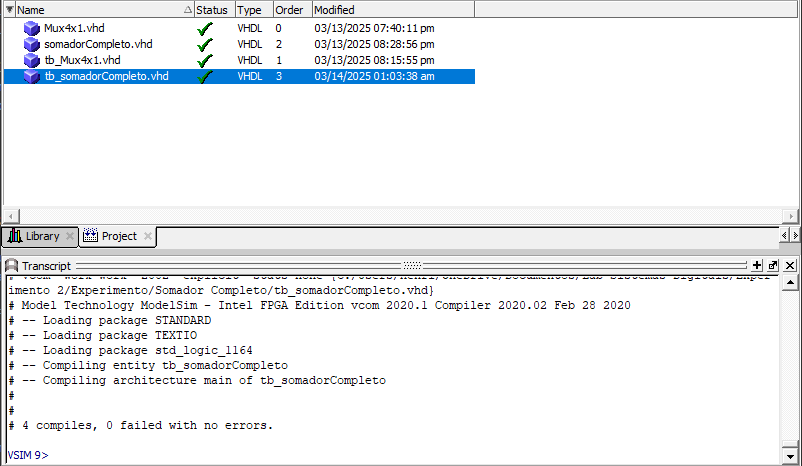
\includegraphics[width=0.75\textwidth]{./Imagens/compileModelSim.png}
    \caption{Compilação do somador completo e seu testbench}
\end{figure}

% Simulação
\section{Simulação}
Após compilar com sucesso os códigos apresentados, deve-se utilizar o ModelSim para testar o funcionamento dos circuitos lógicos correspondentes a eles. Lá, pode-se utilizar a aba "Waves" para analisar o comportamento dos sinais de saída para cada combinação de valores dos sinais de entrada.

Seguem os prints dos resultados das simulações no ModelSim dos códigos apresentados anteriormente:

\begin{figure}[H]
    \centering
    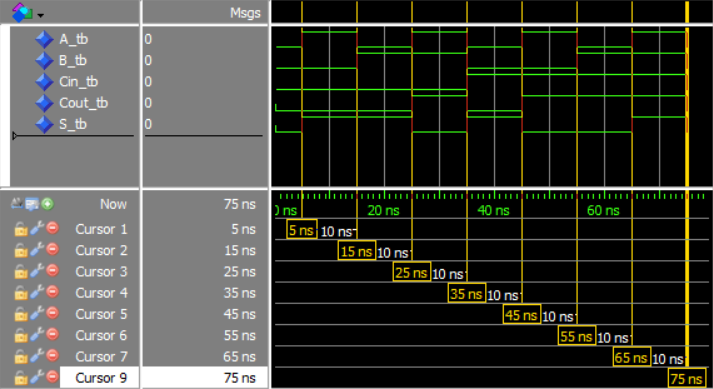
\includegraphics[width=1\textwidth]{Imagens/waves.png}
    \caption{Simulação em forma de onda binária do somador completo}
\end{figure}

\begin{figure}[H]
    \centering
    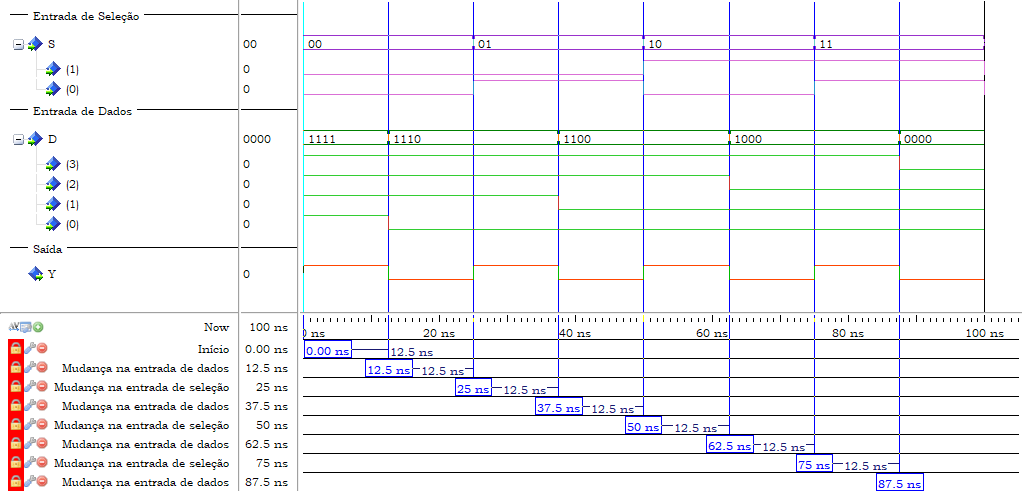
\includegraphics[width=1\textwidth]{Imagens/waves2.png}
    \caption{Simulação em forma de onda binária do multiplexador}
\end{figure}

% Análise
\section{Análise}
Para analisar os resultados obtidos, precisamos apenas mover o cursor na aba "Wave" do ModelSim, assim, conseguimos analisar o valor dos sinais de saída para cada combinação de valores dos sinais de entrada e verificar se os resultados obtidos são os esperados.

A fio, estão exibidos os prints que denotam o comportamento dos sinais de saída para cada possível de estímulo de entrada para o circuito do somador completo.

\begin{figure}[H]
    \captionsetup{skip=0pt} 
    \centering
    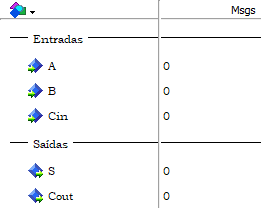
\includegraphics[width=0.35\textwidth]{Imagens/comb1.png}
    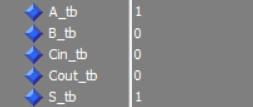
\includegraphics[width=0.35\textwidth]{Imagens/comb2.png}
    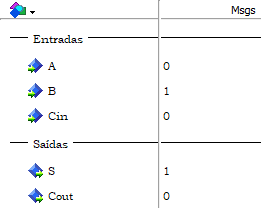
\includegraphics[width=0.35\textwidth]{Imagens/comb3.png}
    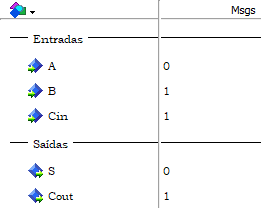
\includegraphics[width=0.35\textwidth]{Imagens/comb4.png}
    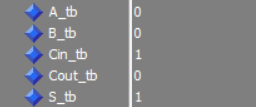
\includegraphics[width=0.35\textwidth]{Imagens/comb5.png}
    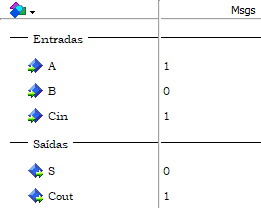
\includegraphics[width=0.35\textwidth]{Imagens/comb6.png}
    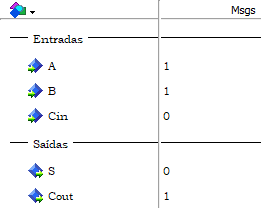
\includegraphics[width=0.35\textwidth]{Imagens/comb7.png}
    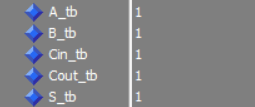
\includegraphics[width=0.35\textwidth]{Imagens/comb8.png}
    \caption{Todas as combinações possíveis de entradas e as saídas correspondentes}
\end{figure}

\noindent Percebe-se que o comportamento está de acordo com o esperado: a concatenação das saídas $C_{out}$ e $S$ corresponde à soma dos bits de entrada $A$, $B$ e $C_{in}$.

Para analisar os resultados para o multiplexador, observou-se o valor da saída $Y$ para cada combinação das entradas de seleção, bem como para cada possível valor da entrada de dados selecionada por cada uma dessas combinações. Abaixo, estão exibidos os prints do comportamento do circuito simulado pelo ModelSim para cada uma dessas combinações. Perceba que cada linha representa uma combinação das entradas de seleção - portanto, uma entrada de dados selecionada - e cada coluna representa um valor para o sinal de entrada de dados selecionado.

\fboxsep=0pt
\begin{longtable}{c@{\hspace{0.15cm}}c}
    \captionsetup{skip=0pt}
    \centering
    \fcolorbox{cinza}{white}{\includegraphics[width=0.35\textwidth]{Imagens/S=00/11.png}} &
    \fcolorbox{cinza}{white}{\includegraphics[width=0.35\textwidth]{Imagens/S=00/00.png}} \\
    \fcolorbox{cinza}{white}{\includegraphics[width=0.35\textwidth]{Imagens/S=10/11.png}} &
    \fcolorbox{cinza}{white}{\includegraphics[width=0.35\textwidth]{Imagens/S=10/00.png}} \\
    \fcolorbox{cinza}{white}{\includegraphics[width=0.35\textwidth]{Imagens/S=01/11.png}} &
    \fcolorbox{cinza}{white}{\includegraphics[width=0.35\textwidth]{Imagens/S=01/00.png}} \\
    \fcolorbox{cinza}{white}{\includegraphics[width=0.35\textwidth]{Imagens/S=11/11.png}} &
    \fcolorbox{cinza}{white}{\includegraphics[width=0.35\textwidth]{Imagens/S=11/00.png}} \\
\caption{Saídas para todas as combinações das entradas de seleção e selecionadas}
\end{longtable}

\noindent Nota-se, em especial, os sinais destacados em cada coluna - sempre o sinal de saída $Y$ e o sinal de entrada selecionado $D_{n}$. É fácil perceber que aquele é igual a este para qualquer combinação das entradas de seleção e valor do sinal selecionado, ou seja, que a saída é igual ao sinal selecionado, como é, por definição, um multiplexador.

% Conclusão
\section{Conclusão}
Nesse experimento, simulou-se, com sucesso, dois dispositivos digitais de suma importância para a eletrônica digital: o somador completo e o multiplexador 4-para-1. No relatório, percebeu-se o sucesso do experimento e pôde-se analisar devidamente os resultados obtidos pelas simulações, por meio das quais foi possível analisar minuciosamente esses dois circuitos e o seu comportamento para cada estímulo possível.

Concluindo, não foram observadas discrepâncias entre o comportamento esperado e o observado, podendo-se concluir, portanto, o sucesso do experimento.

\end{document}